\chapter{Экспериментальный раздел}
Цель экспериментального раздела – пример работы программы, расчет погрешности.

\section{Погрешность измерения размером цилиндра}
Для тестирования было взято три различных цилиндра, сфотографированных с высоты 1 метр 60 сантиметром:
\begin{figure}[H]
	\centering
	\begin{minipage}{.5\textwidth}
		\centering
		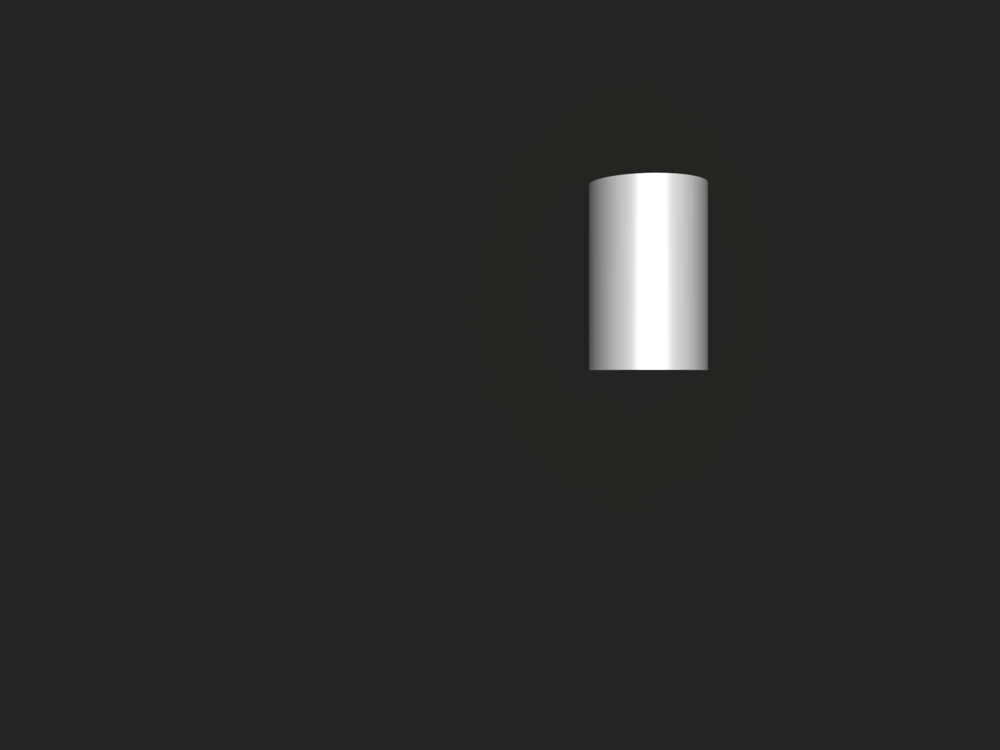
\includegraphics[scale=0.2]{img/16_0045_014.png}
		\caption{Цилиндр 1. Высота 14 сантиметров, радиус 4.5 сантиметра.}
		\label{class:c1}
	\end{minipage}%
	\begin{minipage}{.5\textwidth}
		\centering
		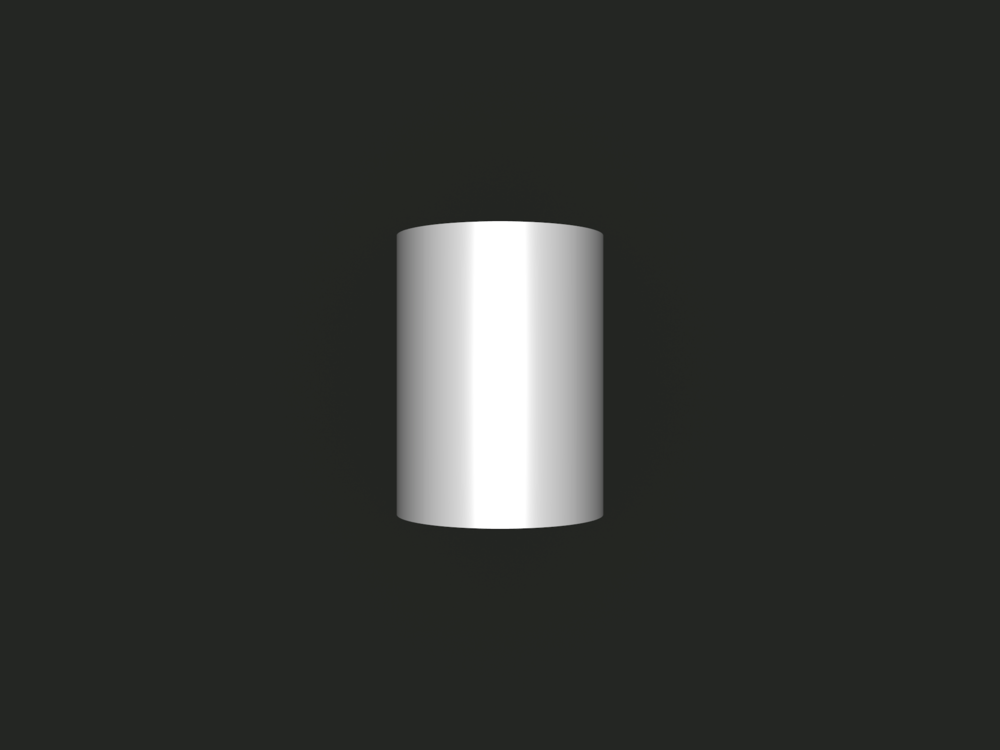
\includegraphics[scale=0.2]{img/16_0075_02.png}
		\caption{Цилиндр 2. Высота 20 сантиметров, радиус 7.5 сантиметра.}
		\label{class:c2}
	\end{minipage}
\end{figure}
\begin{figure}[H]
	\centering

	\begin{minipage}{1\textwidth}
		\centering
		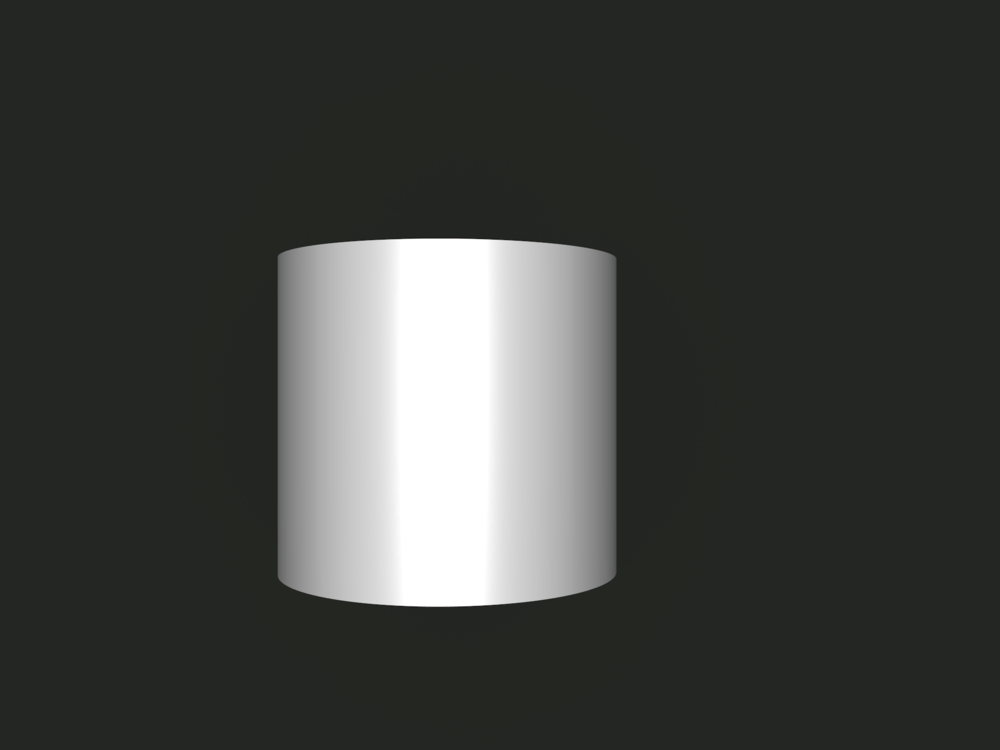
\includegraphics[scale=0.2]{img/16_0115_021.png}
		\caption{Цилиндр 3. Высота 21 сантиметр, радиус 11.5 сантиметра.}
		\label{class:c3}
	\end{minipage}
\end{figure}

В таблице \ref{tbl:1} приведены результаты тестирования:
\begin{table}[H]
	\centering
	\begin{tabular}{|l|l|l|l|l|l|}
		\hline
		\multicolumn{2}{|l|}{\backslashbox{Измерение}{Калибровка}}                                                                    & Цилиндр 1                                                         & Цилиндр 2                                                         & Цилиндр 3                                                         & Отрезок                                                 \\ \hline
		Цилиндр 1 & \begin{tabular}[c]{@{}l@{}}Радиус, м\\ Погрешность, \%\\ Высота, м\\ Погрешность, \%\end{tabular} & \begin{tabular}[c]{@{}l@{}}0.044\\ 1.2\\ 0.14\\ 0\end{tabular}    & \begin{tabular}[c]{@{}l@{}}0.043\\ 4.4\\ 0.136\\ 2.8\end{tabular} & \begin{tabular}[c]{@{}l@{}}0.041\\ 8.8\\ 0.129\\ 8.5\end{tabular} & \begin{tabular}[c]{@{}l@{}}0.046\\ 2.2\\ 0.144\\ 2.8\end{tabular} \\ \hline
		Цилиндр 2 & \begin{tabular}[c]{@{}l@{}}Радиус, м\\ Погрешность, \%\\ Высота, м\\ Погрешность, \%\end{tabular} & \begin{tabular}[c]{@{}l@{}}0.076\\ 1.3\\ 0.205\\ 2.5\end{tabular} & \begin{tabular}[c]{@{}l@{}}0.074\\ 1.3\\ 0.2\\ 0\end{tabular}     & \begin{tabular}[c]{@{}l@{}}0.071\\ 5.3\\ 0.189\\ 5.5\end{tabular} & \begin{tabular}[c]{@{}l@{}}0.78\\ 4.4\\ 0.211\\ 4.4\end{tabular}  \\ \hline
		Цилиндр 3 & \begin{tabular}[c]{@{}l@{}}Радиус, м\\ Погрешность, \%\\ Высота, м\\ Погрешность, \%\end{tabular} & \begin{tabular}[c]{@{}l@{}}0.121\\ 10\\ 0.227\\ 8.2\end{tabular}  & \begin{tabular}[c]{@{}l@{}}0.117\\ 8.3\\ 0.222\\ 5.7\end{tabular} & \begin{tabular}[c]{@{}l@{}}0.112\\ 1.8\\ 0.21\\ 0\end{tabular}    & \begin{tabular}[c]{@{}l@{}}0.124\\ 11.1\\ 0.234\\ 11\end{tabular} \\ \hline
	\end{tabular}
	\caption{Таблица погрешностей}
	\label{tbl:1}
\end{table}

Погрешность можно уменьшить, путем увеличения разрешения изображения, использованием качественных линз, которые дает наименьшую дисторсию, увеличением расстояния между камерой и объектом, чтобы была видна наибольшая часть цилиндра.
\textsl{}